\chapter{Reputation}
\label{ch:reputation}

\symbolfootnote[0]{This chapter reprints material originally
    published as~\cite{Adler2007}.}

\newcommand{\textmass}{\rho_t}
\newcommand{\editmass}{\rho_e}
\newcommand{\specq}{\alpha}
\newcommand{\especq}{\alpha_e}
\newcommand{\tspecq}{\alpha_t}
\newcommand{\repu}{{\text{\textit{rep}}}}
\def\eqpun{\;}
\newcommand{\prece}{{\text{\textit{prec}}}_e}
\newcommand{\prect}{{\text{\textit{prec}}}_t}
\newcommand{\recall}{{\text{\textit{rec}}}}
\newcommand{\recalle}{{\text{\textit{rec}}}_e}
\newcommand{\recallt}{{\text{\textit{rec}}}_t}
\newcommand{\boost}{{\text{\textit{boost}}}}
\newcommand{\booste}{{\text{\textit{boost}}}_e}
\newcommand{\boostt}{{\text{\textit{boost}}}_t}
\newcommand{\constraint}{\kappa}
\newcommand{\constrainte}{\kappa_e}
\newcommand{\constraintt}{\kappa_t}


\section{Introduction}

The problem with modern research trends (Google Pagerank, Netflix
prize, etc) is that we're pursuing human ideas of ``good''.
There is no gold standard, no way to prove correctness except
by example and rhetoric.
This research has the same problem, though we've tried to address
that by having human evaluations and other measures.

The problem of evaluation is also a matter of quality, or at least
putting a quantity on the quality.
In our original work, we propose several ways to do evaluation.
Vandalism includes several different kinds of evaluation.
Problem in our field is that nearly no one does head-to-head
comparisons, so it's legitimate to post some precision/recall
numbers that ``look good'' and then be done with it.

Working in industry, evaluation is also the first thing tossed
out the window in the rush to file patents or create demos.


\section{Related Work}

The work most closely related to ours is \cite{Zeng2006}, where the
revision history of a Wikipedia article is used to compute a trust
value for the article.
Dynamic Bayesian networks are used to model the
evolution of trust level over the versions. 
At each revision, the inputs to the network are a priori models of
trust of authors (determined by their Wikipedia ranks), 
and the amount of added and deleted text. 
The paper shows that this approach can be used to predict the quality
of an article; for instance, it can be used to predict when an article
in a test set can be used as a featured article.  
Differently from the current work, author trustworthiness is
taken as input; we compute author reputation as output. 
Several approaches for computing text trust are outlined
in~\cite{WikiMTWtrust06}. 
A simpler approach to text trust, based solely on text age, is
advocated in~\cite{Cross2006}. 

Document trust, and author reputation, have different applications. 
Document trust provides a measure of confidence in the accuracy of the
document. 
Author reputation is most useful as an indicator of quality
for fresh text, and can be used to manage author activity, for
instance, preventing low-reputation authors from editing some pages. 

Reputation systems in e-commerce and social networks has been extensively
studied~\cite{Kleinberg99,ResnickZFK00,Dellarocas2003,Kamvar2003};
the reputation in those systems is generally user-driven, rather than
content-driven as in our case. 
Related is also work on trust in social networks~\cite{Guha2004,Golbeck2005}. 

The history flow of text contributed by Wikipedia authors has
been studied with flow visualization methods in~\cite{Viegas04}; 
the results have been used to analyze a number of interesting patterns
in the content evolution of Wikipedia articles. 
Work on mining software revision logs~\cite{Livshits05}
is similar in its emphasis of in-depth analysis of revision logs; the
aim, however, is to find revision patterns and indicators that point
to software defects, rather than to develop a notion of author
reputation. 


\section{A Content-Driven Reputation System} 

We propose a \intro{content-driven} reputation system in
order to preserve the current user experience of the Wikipedia.
There are two behaviors that we choose to promote as desirable:
contributing text to articles, and editing text.
Adding text to articles is a necessary behavior for the Wikipedia
to acquire new knowledge and continue to expand.
However, adding text is not sufficient to make the Wikipedia a
useful resource --- the text must be edited for formatting and
readability, and vandalism must be removed, so the removal and
rearrangement of text is also very important.

To measure text contributions and the amount of editing performed
by an author, we examine only the revision history of each article
and use a text differencing algorithm to assist in computing these values.
Deriving implicit judgements from the history was an important
challenge in this work, and our reputation system builds upon
the ideas developed in Chapter~\ref{ch:editquality} for judgements.
Thus, the central premise of our analysis is the notion that later
authors of an article are implicitly judging the work of earlier authors.
In order to reduce the negative impact of vandals, we scale the
computed judgement by the reputation of the judge, so that high-reputation
judges have a larger influence on improving the reputation of the
author being judged.
This limits the damage that vandals can cause by creating multiple
anonymous accounts, and has the side-effect that a user must make
positive contributions that outweigh their negative contributions.

\subsection{Text Contributions} 

We deem a text contribution to be \textit{useful} to the Wikipedia
if it \textit{survives} over multiple revisions.
That is, if later editors choose to preserve the text, then
implicitly they are voting that the contribution was of good
quality.
We would like to increase the reputation of the author making
the text contribution by an amount relative to the size of their
contribution (thus encouraging larger contributions),
but also factoring in the reputation of the judge so as to reduce
the weight of low-reputation users, who might be vandals.

Formally, for an article, $a \in \articles$,
we consider two versions, $\version{i}, \version{j} \in \versions{a}$,
where $i < j$ so that \revauthor{\version{i}} is the author we are
adjusting the reputation of, and \revauthor{\version{j}} is the author
making the implicit judgement.
The amount of text contributed in \version{i} that survives
to \version{j} is then given by \tsurv{a}{i,j}, as defined in
Equation~\ref{eq:tsurv}.
Thus, we propose the following rule:

\begin{regola}
\textbf{(reputation update due to text survival)}
\label{rule-text}
  We update the reputation of \revauthor{\version{i}} by considering
  each of the ten following versions as judges,
  $v_j \in \judges{a}{10}{i}$, and update the reputation by the amount:
  \[
    \coeffrep \cdot \coefftext \cdot \frac{\tsurv{a}{i,j}}{\tsurv{a}{i,i}} 
    \cdot (\tsurv{a}{i,i})^\lengthexp \cdot \log(1 + \rep(\version{j})),
  \]
  where $j = \revpos{\version{j}}$ is the version position of $v$ in \versions{a}
  (and consequently, $0 < j - i \le 10$),
  $\coeffrep > 0$, $\coefftext \in [0,1]$, and $\lengthexp \in
  [0,1]$ are parameters, and where $\rep(\version{j})$ is the reputation of
  \revauthor{\version{j}} at the time \version{j} is performed.
\end{regola}

\noindent
In this rule, $\tsurv{a}{i,j} / \tsurv{a}{i,i}$ is the fraction of text
introduced at version \version{i} that is still present in version \version{j};
this is a measure of the ``quality'' of \version{i}. 
The quantity $\log(1 + \rep(\version{j}))$ is the ``weight'' of the
reputation of \revauthor{\version{j}},
that is, how much the reputation of \revauthor{\version{j}} lends
credibility to the judgements made by \revauthor{\version{j}}. 
In Chapter~\ref{ch:contrib}, we saw that for any measure we investigated,
only a few regular contributors dominate the majority of users by
several orders of magnitude.
We therefore use a logarithmic weight for reputation
to ensure that the feedback coming from new authors is not completely
overridden by the feedback coming from the dominant contributors. 
The parameters $\coeffrep$, $\coefftext$ and $\lengthexp$ were
determined experimentally via an optimization process, described
in Section~\ref{sec:rep-eval}.
The parameter $\lengthexp \in [0,1]$ is an exponent that specifies how
to take into account the length of the original contribution: if
$\lengthexp = 1$, then the increment is proportional to the length of
the original contribution; if $\lengthexp = 0$, then the increment
does not depend on the length of the original contribution.
The parameter $\coeffrep$ specifies how much the reputation should
vary in response to an individual feedback. 
The parameter $\coefftext$ specifies how much the feedback should 
depends on residual text (Rule~\ref{rule-text}) or residual edit
(Rule~\ref{rule-edit}, presented later). 

To give feedback on a revision, the rule considers at most 10
successive versions. 
This ensures that contributors to early versions of articles do not
accumulate disproportionate amounts of reputation. 
We considered basing the limit on time, rather than on the number of
versions, but each Wikipedia article has its own rate of change:
using the number of versions ensures that fast and
slow-changing pages are treated in a similar fashion.

\subsection{Edit Contributions}

Similar to text contributions, we define edit contributions to
be \textit{useful} if they \textit{survive} revision by multiple
later authors.
We use the notion of \intro{edit longevity} defined in
Equation~\ref{eq:esurv} as a guide to the quality judgement
made by \revauthor{\version{j}} of the work by \revauthor{\version{i}}:
\begin{equation*}
\esurv{a}{i,i-1,j} = \frac{\dist{a}{i-1,j} - \dist{a}{i,j}}
                        {\dist{a}{i-1,i}}
\end{equation*}
Intuitively, this formula computes whether the work in going
from version \version{i-1} to version \version{i} brings the
article closer to how the article will look in the future
(as seen from the point of view of version \version{j}).
If the edit distance, $\dist{}{}$,
satisfies the triangular inequality,
then $\esurv{a}{i,i-1,j} \in [-1,1]$;  
we restrict the value of $\esurv{}{}$ to be in this
range by fixing the value to one of the endpoints when
it falls outside of the range.
For two consecutive edits \version{i}, \version{i+1},
if \version{i} is completely undone in \version{i+1}
(as is common when \version{i} introduces spam or is some other
kind of vandalism), then $\esurv{a}{i,i-1,i+1} = -1$; 
if \version{i+1} entirely preserves the work of \version{i},
then $\esurv{a}{i,i-1,i+1} = +1$.
For more distant edits, $\esurv{a}{i,i-1,j}$ is a measure of how much of the
edit performed for version \version{i}
is undone (value $-1$) or preserved (value $+1$) in version \version{j}. 

Note that $\esurv{a}{i,i-1,j} < 0$
only when
$\dist{a}{i-1,i} < \dist{a}{i,j}$,
that is,
when \version{j} is closer to the version \version{i-1}
(the \textit{preceding} version), than to version \version{i}.
In other words, \revauthor{\version{j}}
votes to lower the reputation of \revauthor{\version{i}}
only when the preceding \version{i-1} is more like \version{j}
than \version{i} is.
We use the following rule for updating reputations based on
edit contributions.

\begin{regola}
\textbf{(reputation update due to edit survival)}
\label{rule-edit}
  We update the reputation of \revauthor{\version{i}} by
  using the three following revisions as judges,
  $v_j \in \judges{a}{3}{i}$, to compute the following value:
\begin{equation*}
q = \frac{\slack \cdot \dist{a}{i-1,j} - \dist{a}{i,j}}
                        {\dist{a}{i-1,i}}
\label{eq-edit-long}
\end{equation*}
where $j = \revpos{\version{j}}$.
Since $q$ is undefined when \dist{a}{i-1,i} = 0,
we take that to be a special case where no reputation
should accrue to the author of version \version{i}
(\ie we set $q = 0$ in that case).
We also define a \intro{punishing} function
\begin{equation*}
    p(q) =
        \begin{cases}
            1 & \text{if $q \ge 0$,} \\
            -\coeffpunish & \text{if $q < 0$.} \\
        \end{cases}
\end{equation*}

The reputation of \revauthor{\version{i}} is then increased
according to the following formula:
\begin{equation*}
q \cdot p(q) 
  \cdot \coeffrep \cdot (1 - \coefftext) \cdot 
        (\dist{a}{i-1,i})^\lengthexp \cdot \log(1 + \rep(\version{j}))
\end{equation*}

  In this rule, $\coeffpunish \geq 1$, $\slack \geq 1$, $\coeffrep > 0$, 
  $\coefftext \in [0,1]$, and $\lengthexp \in [0,1]$ are parameters,
  and $\rep(\version{j})$ is the reputation of \revauthor{\version{j}}
  at the time version \version{j} is created.
\end{regola}

We constructed this rule to use a modified form of
Equation~\ref{eq:esurv};
the parameter $\slack > 1$ is used to spare $a_i$ from punishment when
the revision from \version{i-1} to \version{i} is only slightly
counterproductive.
On the other hand, when punishment is incurred, its magnitude is
magnified by the amount $\coeffpunish$, raising the reputation cost of
edits that are later undone. 
We see amplifying the punishment as being instrumental
to making the threat a credible one. 
Without amplification, a rogue contributor could use the reputation
gained in one part of the Wikipedia to constantly destroy a small set
of articles elsewhere.
Amplification makes this harder to achieve. 

The parameters $\slack$ and $\coeffpunish$, as well as $\coeffrep$,
$\coefftext$ and $\lengthexp$, were determined via an optimization
process described in Section~\ref{sec:rep-eval}.

\subsection{Computing Content-Driven Reputation}

We compute the reputation for Wikipedia authors as follows. 
We examine all revisions in chronological order, thus simulating the
same order in which they were submitted to the Wikipedia servers. 
We initialize the reputations of all authors to the value~0.1;
the reputation of anonymous authors is fixed to~0.1.  
We choose a positive initial value to ensure that the weight
$\log (1+r)$ of an initial reputation $r = 0.1$ is non-zero, priming
the process of reputation computation.  
This choice of initial value is not particularly critical (the
parameter $\coeffrep$ may need to be adjusted for optimal performance,
if this initial value is changed). 
As the revisions are processed,we use Rules~\ref{rule-text}
and~\ref{rule-edit} to determine which authors are being
judged by the revision being process,
and update the reputations of those authors accordingly.
When updating reputations, we ensure that they never become negative,
and that they never grow beyond a bound $\coeffmaxrep > 0$. 
The bound $\coeffmaxrep$ prevents frequent contributors from
accumulating unbounded amounts of reputation, and becoming essentially
immune to negative feedback. 
The value of $\coeffmaxrep$ was once again determined via
optimization techniques, as described in Section~\ref{sec:rep-eval}.

Wikipedia allows users to register and create an {\em author\/}
identity whenever (and as often as) they wish. 
As a consequence, we need to make the initial reputation of new authors
very low, close to the minimum possible (in our case,~0). 
If we made the initial reputation of new authors any higher,
then authors, after committing revisions that damage their reputation,
would simply re-register as new users to gain the higher value. 
An unfortunate side-effect of allowing people to obtain new identities
at will is that we cannot presume that people are innocent until
proven otherwise: we have to assign to newcomers the same reputation
as proven offenders.\footnote{Perhaps a way out of this conundrum
is to use the methods of vandalism detectors (discussed
in Section~\ref{sec:vandalism-related}) to determine an
initial reputation based on other factors about the edit.}
This is a contributing factor to our reputation having low 
{\em precision:\/} many authors who have low reputation still perform
very good quality revisions, as they are simply new authors, rather than
proven offenders. 
%% We conjecture that content-driven reputation systems for the Wikipedia
%% would have better predictive value if creating a new author identity
%% was not free, either monetarily, or in some other sense. 



\section{Evaluation Metrics}
\label{sec:rep-eval}

In developing a reputation system, one must ask
``what is it intended to signal?''
For WikiTrust, our hope was that a high reputation
would signal that edits made the author were likely
to be of good quality, while a low reputation would
signal that the edit was of unknown quality.
Evaluation of the system becomes the crucial
factor, so that users can compare one system to another.


At the time that this work was conducted, there was
no annotated corpus of edits available to compare against.
\mynote{Look up what McGuinness did for evaluation in her papers.}

We propose several different metrics for
evaluating our reputation systems, by casting the interpretation
into binary classification problems parameterized by a
quality metric.
We use the two quality metrics explored in Chapter~\ref{ch:editquality}
to define the following categories:
\begin{itemize} 
\item We say that the new text added in version \version{i}
  is \intro{short-lived} if $\quality{tdecay}{10}{i} \leq 0.2$.
  This indicates that at most 20\% of it, on
  average, survives from one version to the next. 

\item We say that the edit performed in taking version
  \version{i-1} to version \version{i}
  is \textit{short-lived} if
  $\quality{elong}{3}{i} \leq -0.8$.

\item We say that a version \version{i} is \intro{low-reputation} if
  $\log (1+\rep(\version{i})) \leq \log(1+\coeffmaxrep) / 5$, indicating that
  the reputation, after logarithmic scaling, falls in the lowest 20\% of
  the range.
  Note that the reputation of \revauthor{\version{i}} does not actually
  change at the time of version \version{i}'s creation; the reputation
  of the author of a revision
  is adjusted as judges become available.

\end{itemize}
We observe that both quality metrics are computed based on the
evolution of the article text \textit{after} the time that
version \version{i} is created, while $\rep(\version{i})$ is
computed based on events \textit{before} the time of \version{i},
so that a comparison between them isn't predisposed to showing
a correlation.


We take the view that revisions are a probabilistic
process, with \versions{} as the set of outcomes across
all articles.
Since we keep only the last revision of several consecutive
versions by the same author, a ``version'' seems somewhat arbitrary.
We therefore weight each version $v \in \versions{}$
(and let $a \in \articles$ be such that $v \in \versions{a}$,
and $i = \revpos{v}$)
by a ``revision amount'' appropriate to the quality being studied:
\begin{itemize}
\item for edit longevity, we weight revisions by
        $\editmass(v) = \dist{a}{i-1,i}$.
\item for text decay, we weight revisions by
        $\textmass(v) = \tsurv{a}{i,i}$.
\end{itemize}


Using our categories as a basis,
we define three random variables $S_e, S_t, L: \versions{}
\mapsto \set{0,1}$ as follows, for all $v \in \versions{}$ where
$i = \revpos{v}$:
%
\begin{itemize} 

\item $S_e(v)=1$ if $\quality{elong}{3}{i} \leq -0.8$, and $S_e(v)=0$ otherwise.
\item $S_t(v)=1$ if $\quality{tdecay}{10}{i} \leq  0.2$, and $S_t(v)=0$ otherwise.
\item $L(v)=1$ if $\log (1+\rep(v)) \leq \log(1+\coeffmaxrep) / 5$,
  and $L(v)=0$ otherwise.

\end{itemize}
%
The {\em precision\/} $\prect$ and {\em recall\/} $\recallt$
for short-lived text, and 
the {\em precision\/} $\prece$ and {\em recall\/} $\recalle$
for short-lived edits, are defined as:
%
\begin{align*}
    \prect & = \textstyle\Pr_t(S_t{=}1 \mid L{=}1) 
  & \recallt & = \textstyle\Pr_t(L{=}1 \mid S_t{=}1) \\
    \prece & = \textstyle\Pr_e(S_e{=}1 \mid L{=}1) 
  & \recalle & = \textstyle\Pr_e(L{=}1 \mid S_e{=}1).
\end{align*}
\begin{comment}
\ifshort
For short-lived text, the {\em precision\/} is 
$
  \textstyle \prect = \Pr_t(S_t=1 \mid L=1)
$,
and the {\em recall\/} is 
$
  \textstyle \recallt = \Pr_t(L=1 \mid S_t=1)
$.
Similarly, for short-lived edits, we define the 
precision is $\prece = \Pr_e(S_e=1 \mid L=1)$, 
and the recall is $\recalle = \Pr_e(L=1 \mid S_e=1)$.
\fi
\end{comment}
These quantities can be computed as usual; for instance, 
\begin{equation*}
  {\textstyle \Pr_e} (S_e=1 \mid L=1) = 
  \frac{\sum_{v \in \versions{}} S_e(v) \cdot L(v) \cdot \editmass(v)}{%
    \sum_{v \in \versions{}} L(v) \cdot \editmass(v)}.
\end{equation*}


We also define: 
%
\begin{align*}
  \booste & = \frac{\Pr_e(S_e=1 \mid L=1)}{\Pr_e(S_e=1)}
            = \frac{\Pr_e(S_e=1 , L=1)}{\Pr_e(S_e=1)\cdot\Pr_e(L=1)} \\
  \boostt & = \frac{\Pr_t(S_t=1 \mid L=1)}{\Pr_t(S_t=1)}
            = \frac{\Pr_t(S_t=1 , L=1)}{\Pr_t(S_t=1)\cdot\Pr_t(L=1)}
\end{align*}
%
Intuitively, $\booste$ indicates how much more likely than average
it is that edits produced by low-reputation authors are short-lived.
The quantity $\boostt$ has a similar meaning. 
Our last indicator of quality are the {\em coefficients of constraint\/}
\[ 
  \constrainte = I_e(S_e,L) / H_e(L)
  \qquad 
  \constraintt = I_t(S_t,L) / H_t(L),
\]
where $I_e$ is the {\em mutual information\/} of $S_e$ and $L$,
computed with respect to $\Pr_e$, and $H_e$ is the entropy of $L$,
computed with respect to $\Pr_e$ \cite{CoverBook}; similarly for
$I_t(S_t,L)$ and $H_t(L)$.
The quantity $\constrainte$ is the fraction of the entropy of the
edit longevity which can be explained by the reputation of the author; 
this is an information-theoretic measure of correlation. 
The quantity $\constraintt$ has an analogous meaning. 

To assign a value to the coefficients $\coeffrep$, $\slack$,
$\coeffpunish$, $\coefftext$, $\lengthexp$, and $\coeffmaxrep$, 
we implemented a search procedure, whose goal was to find values for
the parameters that maximized a given objective function. 
We applied the search procedure to the Italian Wikipedia, reserving
the French Wikipedia for validation, once the coefficients were
determined. 
We experimented with $I_e(S_e,L)$ and $\prece \cdot \recalle$
as objective functions, and they gave very similar results. 


\section{Experimental Results}

To evaluate our content-driven reputation, we considered two Wikipedias: 
%
\begin{itemize}

\item The Italian Wikipedia, consisting of 154,621 articles and 714,280
  {\em filtered\/} revisions; we used a snapshot dated December~11, 2005. 
\item The French Wikipedia, consisting of 536,930 articles and
  4,837,243 {\em filtered\/} revisions; we used a snapshot dated
  October~14, 2006. 

\end{itemize}
%
In both Wikipedias, we studied only \texttt{NS\_MAIN} pages, which
correspond to ordinary articles (other pages are used as comment
pages, or have other specialized purposes). 
Moreover, to allow the accurate computation of our quality
measures which require multiple judges,
we used only revisions that occurred before October~31, 2005 for
the Italian Wikipedia, and before July~31, 2006 for the French one. 
Our algorithms for computing content-driven reputation depend on the
value of six parameters, as mentioned earlier. 
We determined values for these parameters by searching the parameter
space to optimize the coefficient of constraint $\constrainte$, using the Italian
Wikipedia as a training set; the values we determined are: 
%
\begin{align*}
   \coeffrep      & = 13.08
  & \coeffpunish   & = 19.09
  & \lengthexp     & = 0.60   \\
   \slack         & = 2.20
  & \coefftext     & = 0.60
  & \coeffmaxrep   & = 22026
\end{align*}

Figure~\ref{fig:user-breakdown-by-rep} provides a breakdown of
the amount of edits and text additions performed, according to the
reputation of the author.
We find an essentially bimodal distribution:
the overwhelming majority of revisions are authored by the
lowest and highest reputation users in the system.
\mynote{How does this compare with Chapter~5?
How does it compare to other works that describe the
population?}

\begin{figure}
\begin{center}
%GNUPLOT: LaTeX picture with Postscript
\begin{picture}(0,0)%
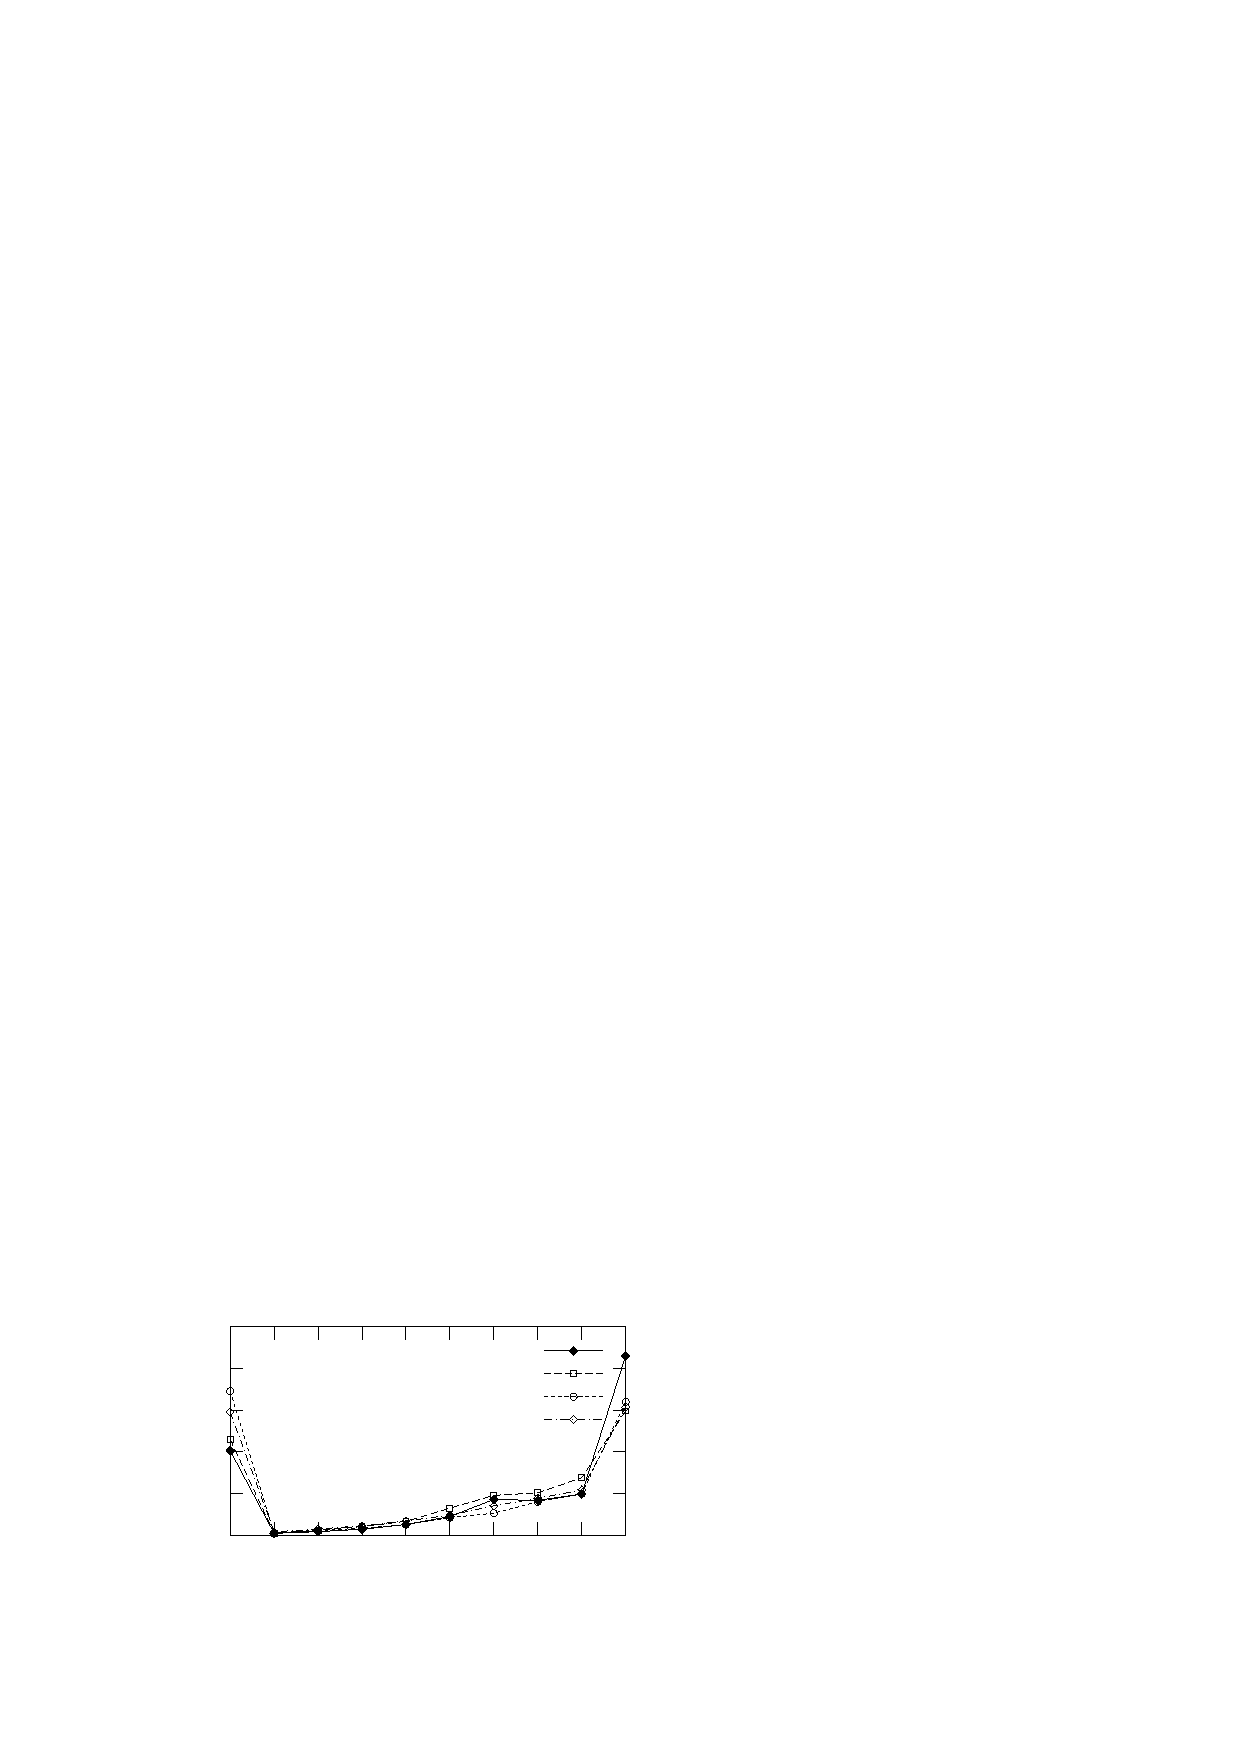
\includegraphics{part-J10-rep/userrep}%
\end{picture}%
\begingroup
\setlength{\unitlength}{0.0200bp}%
\begin{picture}(12240,7200)(0,0)%
\put(1650,1650){\makebox(0,0)[r]{\strut{} 0\%}}%
\put(1650,2650){\makebox(0,0)[r]{\strut{}10\%}}%
\put(1650,3650){\makebox(0,0)[r]{\strut{}20\%}}%
\put(1650,4650){\makebox(0,0)[r]{\strut{}30\%}}%
\put(1650,5650){\makebox(0,0)[r]{\strut{}40\%}}%
\put(1650,6650){\makebox(0,0)[r]{\strut{}50\%}}%
\put(1925,1100){\makebox(0,0){\strut{} 0}}%
\put(2979,1100){\makebox(0,0){\strut{} 1}}%
\put(4034,1100){\makebox(0,0){\strut{} 2}}%
\put(5088,1100){\makebox(0,0){\strut{} 3}}%
\put(6143,1100){\makebox(0,0){\strut{} 4}}%
\put(7197,1100){\makebox(0,0){\strut{} 5}}%
\put(8252,1100){\makebox(0,0){\strut{} 6}}%
\put(9306,1100){\makebox(0,0){\strut{} 7}}%
\put(10361,1100){\makebox(0,0){\strut{} 8}}%
\put(11415,1100){\makebox(0,0){\strut{} 9}}%
\put(6670,275){\makebox(0,0){\strut{}log (1 + reputation)}}%
\put(9190,6075){\makebox(0,0)[r]{\strut{}Italian Wikipedia, edit}}%
\put(9190,5525){\makebox(0,0)[r]{\strut{}Italian Wikipedia, text}}%
\put(9190,4975){\makebox(0,0)[r]{\strut{}French Wikipedia, edit}}%
\put(9190,4425){\makebox(0,0)[r]{\strut{}French Wikipedia, text}}%
\end{picture}%
\endgroup
\endinput

\end{center}
\caption{Percentage of text and edit contributed to the
  Italian and French Wikipedias, according to author reputation. 
  The data includes anonymous authors.}
\label{fig:user-breakdown-by-rep}
\end{figure}


\subsection{Precision and Recall}

We analyzed the Italian and French Wikipedias using the
parameter values discovered by our optimization procedure.
The results are summarized in Table~\ref{tbl:summary-results}. 
The results are better for the larger French Wikipedia; in particular,
the reputation's ability to predict short-lived edits is better on the
French than on the Italian Wikipedias. 
We are not sure whether this depends on different dynamics in the two
Wikipedias, or whether it is due to the greater age (and size) of the
French Wikipedia.
We see that edits performed by low-reputation authors are four times
as likely as the average to be short-lived. 

\begin{sidewaystable}[tp]
\begin{center}
\begin{tabular}{|r||c|c||c|c||c|c||c|c|} \hline
 & \multicolumn{2}{|c||}{Precision}
 & \multicolumn{2}{|c||}{Recall}
 & \multicolumn{2}{|c||}{Boost}
 & \multicolumn{2}{|c|}{Coeff.\ of constr.} \\
 & Edit & Text & Edit & Text  & Edit & Text & Edit & Text \\
 & $\prece$ & $\prect$ & $\recalle$ & $\recallt$ & $\booste$ & $\boostt$ 
 & $\constrainte$ & $\constraintt$ \\[0.5ex] \hline 
\textbf{Excluding anonymous authors: \quad} & & & & & & & & \\
\qquad French Wikipedia          & 23.92\% &  5.85\% & 32.24\% & 37.80\% & $4.21\times$ & $4.51\times$ &  7.33 &  6.29 \\
\qquad Italian Wikipedia         & 14.15\% &  3.94\% & 19.39\% & 38.69\% & $4.03\times$ & $5.83\times$ &  3.35 &  7.17 \\ \hline
\textbf{Including anonymous authors: \quad} & & & & & & & & \\
\qquad French Wikipedia          & 48.94\% & 19.01\% & 82.86\% & 90.42\% & $2.35\times$ & $2.97\times$ & 25.29 & 23.00 \\
\qquad Italian Wikipedia         & 30.57\% &  7.64\% & 71.29\% & 84.09\% & $3.43\times$ & $3.58\times$ & 19.83 & 17.49 \\ \hline
\end{tabular}
\end{center}
\caption{Summary of the performance of content-driven reputation for
the Italian and French Wikipedias.}
\label{tbl:summary-results}
\end{sidewaystable}


\subsection{Manual Annotation}

To investigate how many of the edits had a short life due to bad quality,
we asked a group of seven volunteers to rate revisions made to the
Italian Wikipedia. 
We selected the revisions to be ranked so that they contained
representatives of all 4 combinations of high/low reputation author,
and high/low longevity. 
We asked the volunteers to rate the revisions with $+1$ (good), 
$0$ (neutral), and $-1$ (bad); in total, 680 revisions
were ranked. 
The results, summarized in Table~\ref{tbl:human}, are striking. 
Of the short-lived edits performed by low-reputation users, fully
66\% were judged bad. 
On the other hand, less than 19\% of the short-lived edits performed by
high-reputation users were judged bad. 
We analyzed in detail the relationship between user reputation, and
the percentage of short-lived text and edits that users considered bad. 
Using these results, we computed the approximate recall factors on the
Italian Wikipedia of content-driven reputation for {\em bad\/} edits,
as judged by users, rather than short-lived ones:
%
\begin{itemize}

\item The recall for short-lived edits that are judged to be bad is over
  49\%.

\item The recall for short-lived text that is judged to be bad is over
  79\%.

\end{itemize}
%
These results clearly indicate that our content-driven reputation is a
very effective tool for spotting, at the moment they are introduced,
bad contributions that will later be undone. 
There is some margin of error in this data, as our basis for
evaluation is a small number of manually-rated revisions, and human
judgement on the same revisions often contained discrepancies. 

The fact that so few of the short-lived edits performed by
high-reputation authors were judged to be of bad quality points to the
fact that edits can be undone for reasons unrelated to quality. 
Many Wikipedia articles deal with current events; edits to those
articles are undone regularly, even though they may be of good
quality. 
Our algorithms do not treat in any special way current-events pages. 
Other Wikipedia edits are administrative in nature, flagging pages that
need work or formatting; when these flags are removed, we classify it
as text deletion. 
Furthermore, our algorithms do not track text across articles, so that
when text is moved from one article to another, it is classified as
deleted from the source article.

From Table~\ref{tbl:summary-results}, we note that the precision is
low, by search standards.
Our problem, however, is a prediction problem, not a retrieval
problem, and thus it is intrinsically different. 
The group of authors with low reputation includes many authors who are
good contributors, but who are new to the Wikipedia, so that they have
not had time yet to build up their reputation.


\begin{table}
\begin{center}
\begin{tabular}{|r|c|c|} \hline
\qquad \qquad Reputation & Judged bad & Judged good \\ \hline
\multicolumn{1}{|l|}{Short-lived edits: \qquad \quad} & & \\[1ex]
   Low [0.0--0.2]   &    66  \% &    19 \% \\
Normal [0.2--1.0]   &    16  \% &    68 \% \\ \hline
\multicolumn{1}{|l|}{Short-lived text: \qquad \quad} & & \\[1ex]
   Low [0.0--0.2]   &    74  \% &    13 \% \\
Normal [0.2--1.0]   &    14  \% &    85 \% \\ \hline
\end{tabular}
\end{center}
\caption{User ranking of short-lived edits and text, as a
  function of author reputation, for the Italian Wikipedia.  
  We presented edit differences to a test group of users,
  and asked users to rate whether the edit was good or bad.
  In square brackets, we give the
  interval where the normalized value $\log(1+r) / \log (1 +
  \coeffmaxrep)$ of a reputation $r$ falls.  The precentages do not
  add to 100\%, because users could also rank changes as ``neutral''.} 
\label{tbl:human}
\end{table}

\subsection{Comparison with Edit-Count Reputation}

\begin{sidewaystable}
\begin{center}
\begin{tabular}{|l||c|c||c|c||c|c||c|c|} \hline
 & \multicolumn{2}{|c||}{Precision}
 & \multicolumn{2}{|c||}{Recall}
 & \multicolumn{2}{|c||}{Boost}
 & \multicolumn{2}{|c|}{Coeff.\ of constr.} \\
 & Edit & Text & Edit & Text  & Edit & Text & Edit & Text \\
 & $\prece$ & $\prect$ & $\recalle$ & $\recallt$ & $\booste$ & $\boostt$ 
 & $\constrainte$ & $\constraintt$ \\[0.5ex] \hline 
\textbf{Italian Wikipedia:} & & & & & & & & \\
\qquad Content-driven reputation & 14.15 &  3.94 & 19.39 & 38.69 & 4.03 & 5.83 & 3.35 & 7.17 \\
\qquad Edit count as reputation  & 11.50 &  3.32 & 19.09 & 39.52 & 3.27 & 4.91 & 2.53 & 6.35 \\ \hline
\textbf{French Wikipedia:} & & & & & & & & \\
\qquad Content-driven reputation & 23.92 &  5.85 & 32.24 & 37.80 & 4.21 & 4.51 & 7.33 & 6.29 \\
\qquad Edit count as reputation &  21.62 &  5.63 & 28.30 & 37.92 & 3.81 & 4.34 & 5.61 & 6.08 \\ \hline
\end{tabular}
\end{center}
\caption{Summary of the performance of content-driven reputation over
the Italian and French Wikipedias. All data are expressed as
percentages. Anonymous authors are not included in the comparison.
Precision is the probability that the text or edit longevity is low,
given that the reputation is low.
Recall is the probability that the reputation is low, given
that the text or edit longevity is low.
}
\label{tbl:comparison-with-count} 
\end{sidewaystable}

\mynote{Double-check the results of Halfaker2011 with this next
``commonly believed'' statement.}

We compared the performance of our content-driven reputation to 
another basic form of reputation: {\em edit count.} 
It is commonly believed that, as Wikipedia authors gain experience
(through revision comments, talk pages, and reading articles on
Wikipedia standards), the quality of their submissions goes up.
Hence, it is reasonable to take edit count, that is, the number of
edits performed, as a form of reputation. 
We compare the performance of edit count, and of content-driven
reputation, in Table~\ref{tbl:comparison-with-count}. 
The comparison does not include anonymous authors, as we do not have a
meaningful notion of edit-count for them. 
According to our metrics, content-driven reputation
performs slightly better than edit-count reputation on both the Italian 
and French Wikipedias. 

\mynote{Again, double-check with Halfaker2011.}
We believe that one reason edit-count based reputation performs well
in our measurements is that authors, after performing edits that are
often criticized and reverted, commonly either give up their identity
in favor of a ``fresh'' one, thus zeroing their edit-count reputation
(thus ``punishing'' themselves), or stop contributing to the
Wikipedia. 
However, we believe that the good performance of edit count is an
artifact, due to the fact that edit count is applied to an
already-existing history of contributions. 
Were it announced that edit count is the chosen notion of reputation,
authors would most likely modify their behavior in a way that both
rendered edit count useless, and damaged the Wikipedia. 
For instance, it is likely that, were edit count the measure of
reputation, authors would adopt strategies (and automated robots) for
performing very many unneeded edits to the Wikipedia, causing
instability and damage. 
In other words, edit count as reputation measure has very little
prescriptive value. 
In contrast, we believe our content-driven reputation, by prizing
long-lasting edits and content, would encourage constructive behavior
on the part of the authors. 

\subsection{Text Age and Author Reputation as Trust Criteria}

The age of text in the Wikipedia is often considered as an
indicator of text trustworthiness, the idea being that text that has
been part of an article for a longer time has been vetted by more
contributors, and thus, it is more likely to be correct~\cite{Cross2006}. 
We were interested in testing the hypothesis that author reputation,
in addition to text age, can be a useful indicator of
trustworthiness, especially for text that has just been added to a
page, and thus that has not yet been vetted by other contributors.
Let {\em fresh text\/} be the text that has just been inserted in a
Wikipedia article. 
We considered all text that is fresh in all the Italian
Wikipedia, and we measured that 3.87~\% of this fresh text is deleted
in the next revision.  In other words,
$\Pr(\mbox{deleted}\mid\mbox{fresh}) = 0.0387$. 
We then repeated the measurement for text that is both fresh, and is
due to a low-reputation author: 6.36~\% of it was deleted in the next
revision, or 
$\Pr(\mbox{deleted}\mid\mbox{fresh and low-reputation}) = 0.0636$. 
This indicates that author reputation is a useful factor in predicting
the survival probability of fresh text, if not directly its
trustworthiness. 
Indeed, as remarked above, since text can be deleted for a number of
reasons aside from bad quality, author reputation is most likely a
better indicator of trustworthiness than these figures indicate. 


\subsection{Conclusions}

After comparing edit and text longevity values with user quality
ratings for revisions, we believe that the largest residual source of
error in our content-driven reputation lies in the fact that our text
analysis does not include specific knowledge of the Wikipedia markup
language and Wikipedia conventions. 

%% It is occasionally claimed that the reputation of Wikipedia authors
%% should be domain-specific, so that a good reputation for writing about
%% mathematics does not automatically translate to a good reputation for
%% writing about history. 
%% We are not sure domain-specific reputation has more prediction value 
%% than generic reputation, such as the one we build in this paper.
%% We suspect that a sense of one's own abilities and limitations, and a
%% knowledge of Wikipedia customs, may play a more important role than
%% domain-specific knowledge in determining the average quality of an
%% author's contributions. 
%% The techniques developed for this paper enable us to easily measure
%% the contributions of authors to various categories of the Wikipedia,
%% so we plan to study the usefulness of domain-specific reputation from
%% an experimental point of view in future work.

%\section{Cut Results}

% This is stuff that I cut from results.tex for clarity, but that I
% wanted to preserve.  Note that in any case, much data is in the
% research wiki. Luca


\begin{sidewaystable}
\begin{center}
\begin{tabular}{|r|r||r|r|r|r|r|r|r|r|r|r|r|}
\hline
 & & \multicolumn{11}{|c|}{Cumulative Distribution of Edit Count over Edit Longevity} \\
 \hline
\textbf{Rep}   & \textbf{\%data}
& \textbf{$\le 1.0$} & \textbf{$\le 0.8$}   & \textbf{$\le 0.6$}   & \textbf{$\le 0.4$}   & \textbf{$\le 0.2$}   & \textbf{$\le 0.0$}   & \textbf{$\le -0.2$}  & \textbf{$\le -0.4$} & \textbf{$\le -0.6$}   & \textbf{$\le -0.8$}  & \textbf{$\le -1.0$}\\
\hline
\hline
0.0   &  1.72  &  100 & 30.491 & 26.889 & 25.107 & 23.941 & 23.716 & 23.325 & 23.117 & 22.080 & 21.600 &  9.689 \\
1.0   &  4.11  &  100 & 33.577 & 30.432 & 16.977 & 16.488 & 15.996 & 14.996 & 14.607 &  7.597 &  7.264 &  2.592 \\
2.0   &  4.11  &  100 & 12.878 &  9.987 &  8.405 &  8.024 &  7.497 &  7.214 &  6.323 &  5.537 &  5.276 &  1.694 \\
3.0   &  5.49  &  100 & 10.250 &  7.184 &  5.860 &  5.153 &  4.606 &  4.285 &  3.931 &  2.818 &  2.473 &  0.553 \\
4.0   &  7.78  &  100 & 11.608 &  7.588 &  5.768 &  5.160 &  4.358 &  4.002 &  3.503 &  2.669 &  1.860 &  0.734 \\
5.0   &  10.77 &  100 & 12.216 &  8.232 &  6.280 &  5.327 &  4.773 &  4.317 &  3.750 &  2.422 &  1.770 &  0.530 \\
6.0   &  11.38 &  100 & 16.730 & 12.216 &  8.407 &  7.316 &  6.681 &  5.555 &  4.895 &  3.580 &  3.181 &  0.668 \\
7.0   &  13.86 &  100 & 15.810 & 12.371 & 10.121 &  9.402 &  8.911 &  8.342 &  7.856 &  6.129 &  3.743 &  0.486 \\
8.0   &  17.26 &  100 & 14.768 & 12.640 & 11.071 & 10.290 &  9.858 &  9.246 &  8.641 &  7.338 &  5.358 &  0.830 \\
9.0   &  16.72 &  100 & 10.484 &  7.978 &  6.268 &  4.991 &  4.369 &  3.886 &  3.194 &  2.304 &  1.967 &  0.311 \\
10.0  &  6.80  &  100 &  2.923 &  1.896 &  1.439 &  1.203 &  1.068 &  0.902 &  0.536 &  0.357 &  0.268 &  0.103 \\
\hline
\end{tabular}
\caption{Cumulative distribution of revisions over edit longevity, grouped by edit count reputation.
    Each row shows how many of the total revisions were edited by users of each
    reputation range (the ``\%data'' column), and how that subset of revisions
    was distributed when ranked by edit longevity.}
\end{center}
\label{tbl:edit-count-over-edit-long}
\end{sidewaystable}



Our evaluation of ``edit count'' when compared against
edit longevity is shown in
Table~\ref{tbl:edit-count-over-edit-long},
which allows us to directly read the probability
of edit longevity judging an edit as bad
(the precision of the reputation function)
is 21.6\% for the lowest reputation users,
or 11.5\% if we consider the two lowest
rankings of reputation.
% (1.72 * .2160 + 4.11 * .07264) / (1.72 + 4.11) == 11.5%
Calculating the data density for edits
where the edit longevity is less than or
equal to -0.8, we find that 19\%
of the bad edits are performed
by users with a low reputation
(the recall of the reputation function).




\iflong

\begin{table*}
\begin{center}
\begin{tabular}{|r|r||r|r|r|r|r|r|r|r|r|r|r|}
\hline
 & & \multicolumn{11}{|c|}{Distribution of Edit Longevity over Edit Count} \\
 \hline
\textbf{Rep}   & \textbf{\%data}
& \textbf{$1.0$} & \textbf{$0.8$}   & \textbf{$0.6$}   & \textbf{$0.4$}   & \textbf{$0.2$}   & \textbf{$0.0$}   & \textbf{$-0.2$}  & \textbf{$-0.4$} & \textbf{$-0.6$}   & \textbf{$-0.8$}  & \textbf{$-1.0$}\\
\hline
\hline
0.0   &  1.71   &   1.382 &  1.938 &  1.248 &  2.637 &  0.737 &  1.190 &  0.611 &  1.155 &  0.858 &  7.561 & 20.497 \\
1.0   &  4.14   &   3.181 &  4.529 & 23.281 &  2.728 &  3.628 &  8.093 &  2.775 & 20.320 &  2.077 &  7.069 & 12.541 \\
2.0   &  4.20   &   4.251 &  3.822 &  2.679 &  2.128 &  5.900 &  2.197 &  6.400 &  2.185 &  1.111 &  5.380 &  8.590 \\
3.0   &  5.70   &   5.955 &  5.461 &  3.270 &  3.817 &  6.388 &  3.505 &  3.278 &  4.500 &  1.900 &  4.014 &  3.528 \\
4.0   &  7.90   &   8.116 & 10.497 &  5.835 &  5.200 & 12.188 &  5.129 &  7.116 &  4.721 &  6.245 &  3.133 &  6.986 \\
5.0   &  10.84  &  11.067 & 13.585 &  8.627 & 12.421 & 10.313 &  9.001 & 11.518 & 10.249 &  7.105 &  5.240 &  7.009 \\
6.0   &  11.59  &  11.261 & 16.254 & 17.328 & 15.431 & 15.012 & 23.129 & 11.984 & 11.018 &  4.605 & 10.840 &  8.730 \\
7.0   &  13.91  &  13.586 & 15.744 & 12.963 & 12.151 & 12.064 & 13.115 & 11.796 & 17.298 & 34.260 & 17.188 &  8.201 \\
8.0   &  17.03  &  16.787 & 12.424 & 11.656 & 16.468 & 13.390 & 18.185 & 18.990 & 17.000 & 35.392 & 28.911 & 16.736 \\
9.0   &  16.18  &  16.756 & 13.519 & 11.748 & 25.077 & 18.866 & 14.402 & 20.988 & 10.705 &  5.832 & 10.255 &  6.368 \\
10.0  &  6.80   &   7.657 &  2.228 &  1.365 &  1.941 &  1.515 &  2.053 &  4.544 &  0.849 &  0.617 &  0.408 &  0.813 \\
\hline
\end{tabular}
\caption{Columns sum to 100\%.}
\end{center}
\end{table*}

\fi

\section{Conclusions}

We propose two measures of revision quality computed
from Wikipedia's revision history.
The measure \textit{text longevity} is based on an intuitive
model of computing the text added by authors at each revision
and detecting how much of that text remains within the article
in subsequent revisions; to account for the variation in
the amount of preserved text over the subsequent revisions,
we model the change as a geometrically decaying process
and compute the decay rate as a single value to describe
the variation.
The measure \textit{edit longevity} was developed to address
the reality that authors also delete and rearrange text,
and that these are valuable contributions to the Wikipedia.
We use edit distance~\cite{Levenshtein1966} to describe the
amount of \intro{effort} that an author puts into making a
revision to an article; this is the basis for computing
edit longevity, which estimates the amount of effort by an
author that brings the article text closer to some future
version of the article.

We evaluate these two measures using the PAN-WVC-10 dataset, which is
manually annotated to indicate which revisions are vandalism and which
are well-intentioned edits, and treat each as a predictor of vandalism.
We find that edit longevity performs much better than text longevity,
but even text longevity does better than chance at predicting vandalism.
Overall, these results are encouraging for using edit longevity and text
longevity as signals for inferring the community feedback of an author's
edit.  Knowing the quality of edits, we can build an author reputation
system upon these signals; we describe such a system in
Chapter~\ref{ch:reputation}.



